
\FloatBarrier\begin{figure}[!h]
\centering
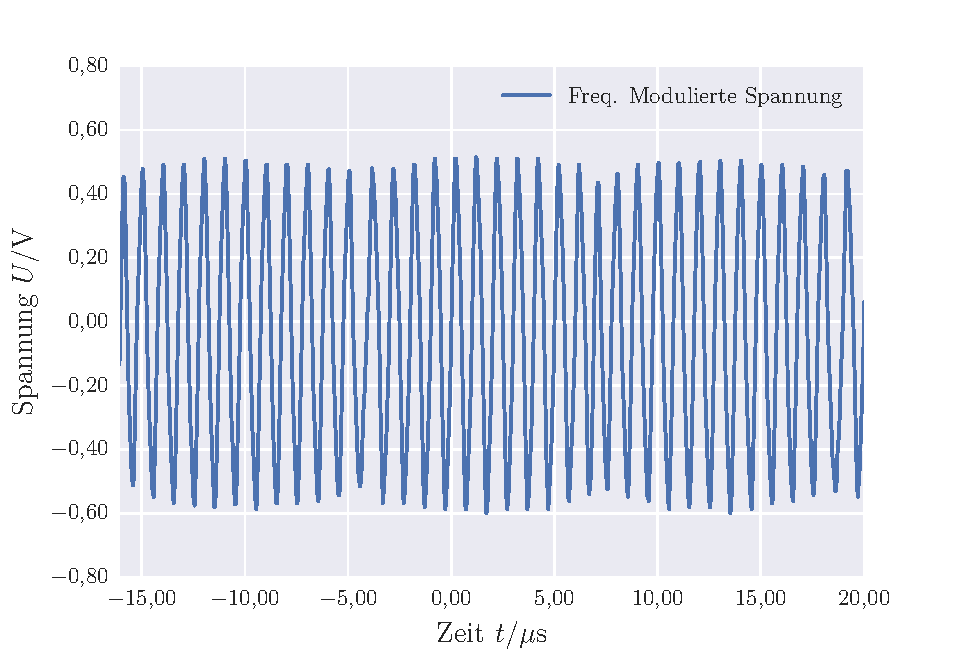
\includegraphics[scale=1]{../Grafiken/Frequenz_Modulierte_Spannung.pdf}
\caption{Frequenzmodulierte Spannung die durch Addition der Seitenbänder aus einer Amplitudenmodulation
	mit Trägerunterdrückung und der phasenverschobenen Trägerspannung erzeugt wurde. Neben der schwachen 
	Frequenzmodulation ist zusätzlich eine geringe Amplitudenmodulation festzustellen.  \label{fig:frequenz_modulierte_spannung}}
\end{figure}
\FloatBarrier